\documentclass[main.tex]{subfiles}
\begin{document}

% ── Block 0: The Limits of TWFE, and Why We Need Three New Toolkits ──────
\section{The Limits of TWFE}

% ── Frame 1: The clean case ─────────────────────────────────────────────
\begin{frame}{The Clean Case: DiD 2$\times$2}

  \begin{columns}[T]
    \begin{column}{0.48\textwidth}
      Two groups, two periods:
      \begin{itemize}
        \item One group treated at $t=1$, the other never
        \item The causal effect is a \emph{double difference}
      \end{itemize}

      \medskip
      \begin{equation*}
        \widehat{\delta} =
          \underbrace{\bigl(\bar{Y}^{\text{tr}}_{\text{post}}
                          - \bar{Y}^{\text{tr}}_{\text{pre}}\bigr)}_{\text{change in treated}}
          -
          \underbrace{\bigl(\bar{Y}^{\text{co}}_{\text{post}}
                          - \bar{Y}^{\text{co}}_{\text{pre}}\bigr)}_{\text{change in control}}
      \end{equation*}

      \medskip
      The first difference wipes out fixed level gaps.
      The second wipes out the common time trend.
    \end{column}
    \begin{column}{0.48\textwidth}
      \begin{tikzpicture}[scale=0.85]
        \draw[->] (0,0) -- (3.2,0) node[right]{\small time};
        \draw[->] (0,0) -- (0,3.2) node[above]{\small outcome};
        \node[below] at (1,0) {\small Pre};
        \node[below] at (2.5,0) {\small Post};
        \draw[dashed,gray] (1,-0.1) -- (1,3.0);
        \draw[color=MidBlue,thick] (1,1.0) -- (2.5,1.8)
          node[right]{\small\color{MidBlue}Control};
        \fill[MidBlue] (1,1.0) circle (2pt);
        \fill[MidBlue] (2.5,1.8) circle (2pt);
        \draw[color=DarkBlue,thick] (1,1.5) -- (2.5,3.0)
          node[right]{\small\color{DarkBlue}Treated};
        \fill[DarkBlue] (1,1.5) circle (2pt);
        \fill[DarkBlue] (2.5,3.0) circle (2pt);
        \draw[color=DarkBlue,dashed] (1,1.5) -- (2.5,2.3);
        \fill[DarkBlue,opacity=0.4] (2.5,2.3) circle (2pt);
        \draw[<->,AlertRed,thick] (2.5,2.3) -- (2.5,3.0)
          node[midway,right]{\small\color{AlertRed}ATT};
      \end{tikzpicture}
    \end{column}
  \end{columns}

  \medskip
  \textbf{Key assumption:} \alert{parallel trends} --- absent treatment, both
  groups would have moved \emph{in parallel}. Levels may differ; only the
  \emph{slopes} must match. This is a claim about a \emph{counterfactual},
  so in a 2$\times$2 you cannot test it --- you assume it.

\end{frame}

% ── Frame 2: From 2x2 to TWFE ───────────────────────────────────────────
\begin{frame}{From the 2$\times$2 to TWFE}

  In the 2$\times$2 world, the DiD estimate is the coefficient $\beta_3$ in:
  \begin{equation*}
    Y_{it} = \beta_0 + \beta_1\,\text{Post}_t + \beta_2\,\text{Treated}_i
             + \beta_3\,(\text{Post}_t \times \text{Treated}_i) + \varepsilon_{it}
  \end{equation*}

  With a panel of many units and periods, researchers run the natural
  generalisation --- \alert{two-way fixed effects}:
  \begin{equation*}
    Y_{it} = \alpha_i + \lambda_t + \beta\,D_{it} + \varepsilon_{it}
    \qquad\text{($\alpha_i$: unit FE, \ \ $\lambda_t$: time FE)}
  \end{equation*}

  \medskip
  Here $\beta$ plays the role of $\beta_3$: it is \emph{supposed} to be the ATT.
  In 2010--2012, 19\% of empirical AER articles used it (dCH, 2020).

  \medskip
  \begin{alertblock}{An assumption that usually stays implicit}
    If the effect is \alert{the same in every $(g,t)$ cell}, $\hat\beta$
    equals it in any design. Otherwise it is a weighted sum of cell effects
    (weights sum to one, \alert{can be negative}), equal to the ATT only if
    weights and effects are uncorrelated. The rest of
    this block is \emph{when} that matters, and \emph{which toolkit} fixes each case.
  \end{alertblock}

\end{frame}

% ── Frame 3: When is TWFE actually fine? (misconception buster) ──────────
\begin{frame}{First, the Honest Part: When \emph{Is} TWFE Fine?}

  TWFE estimates a \alert{weighted sum} of the cell effects $\Delta_{g,t}$
  (cohort $g$, period $t$); the weights sum to one but \alert{can be negative}.
  Two situations make it trustworthy:

  \medskip
  \begin{columns}[T]
    \begin{column}{0.5\textwidth}
      \begin{block}{Two routes to safety}
        \begin{itemize}
          \item \textbf{Homogeneous effects.} If $\Delta_{g,t}$ is the same in
            every cell, the weighted sum equals it \emph{exactly} --- in
            \emph{any} design.
          \item \textbf{Clean design.} Binary treatment, one adoption date,
            nobody treated before it: every treated cell gets the \alert{same}
            weight. (Two periods alone are not enough.)
        \end{itemize}
      \end{block}
    \end{column}
    \begin{column}{0.5\textwidth}
      \begin{alertblock}{Bias, and sign reversal}
        \begin{itemize}
          \item \textbf{Bias}: effects that \textbf{vary} (by cohort or over
            time), \textbf{correlated with the TWFE weights}.
          \item A \textbf{sign flip} also needs \textbf{negative weights},
            possible with \textbf{staggered} timing, \textbf{on/off} switching
            or \textbf{non-binary} treatment.
        \end{itemize}
        Then a positive effect can enter with a negative weight, and
        $\hat\beta$ shrinks or flips sign.
      \end{alertblock}
    \end{column}
  \end{columns}

  \medskip
  \footnotesize Homogeneous effects (any design) or a clean design (any
  heterogeneity): $\hat\beta$ is the ATT. Staggered dates, effects differing by
  cohort: a variance-weighted ATT, plus a bias term if effects change over time.

\end{frame}

% ── Frame 4: TWFE = weighted average of 2x2's ───────────────────────────
\begin{frame}{What TWFE Really Computes: A Weighted Average of 2$\times$2's}

  \textbf{Goodman-Bacon (2021)} proves that with binary, staggered treatment:
  \begin{equation*}
    \hat{\beta}^{\text{TWFE}}
      = \sum_{(k,\ell)} s_{k\ell}\;\hat{\delta}^{\,2\times2}_{k\ell}
  \end{equation*}

  $\hat{\beta}^{\text{TWFE}}$ is a \alert{weighted average of every possible
  2$\times$2 DiD} between two timing groups (the never-treated included). Each
  2$\times$2 compares average outcomes over two time windows set by the adoption
  dates (before, between and after adoption), not two single dates.

  \medskip
  What matters is which comparisons enter that average. Some are clean. One
  compares a newly-treated group to a group \emph{that is already treated} ---
  and \emph{when effects change over time}, that comparison is what biases
  $\hat\beta$.

\end{frame}

% ── Frame 5: The four comparisons (Bacon figure) ────────────────────────
\begin{frame}{The Four Comparisons Behind $\hat\beta^{\text{TWFE}}$}

  \begin{columns}[T]
    \begin{column}{0.62\textwidth}
      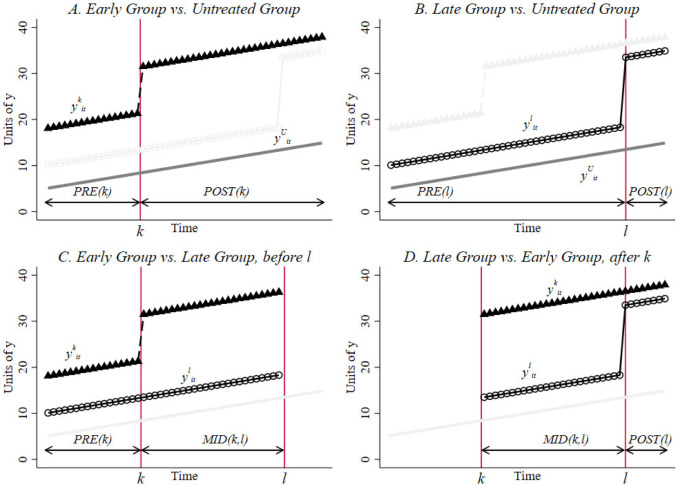
\includegraphics[width=\textwidth]{figures/block0/bacon_comparisons.jpg}
    \end{column}
    \begin{column}{0.36\textwidth}
      \footnotesize
      \textbf{A, B} --- early/late treated vs.\ \emph{never-treated}.
      \textcolor{MidBlue}{Clean controls.}

      \medskip
      \textbf{C} --- early vs.\ late, \emph{before} the late group is treated.
      The late group is still untreated, so \textcolor{MidBlue}{also a clean control.}

      \medskip
      \textbf{D} --- late vs.\ early, \emph{after} the early group is treated.
      Now the ``control'' \alert{already has the treatment}.
      \alert{This is the forbidden comparison.}
    \end{column}
  \end{columns}

  \medskip
  \footnotesize\itshape Goodman-Bacon (2021), \textit{J.\ Econometrics}, Fig.~2.
  Dark series: the data each 2$\times$2 uses; faded grey: left out.

\end{frame}

% ── Frame 6: The forbidden comparison in plain English → Block 1 ─────────
\begin{frame}{Failure \#1: The Forbidden Comparison \hfill {\small$\rightarrow$ Block 1}}

  \begin{columns}[T]
    \begin{column}{0.55\textwidth}
      Think of a reform rolled out in waves --- say no-fault divorce laws,
      adopted by early states and, years later, by late states.

      \medskip
      To estimate the \emph{late} states' effect, TWFE needs a control for them.
      Panel~D used the \alert{early states} --- but by then they have had
      the law for years. Their outcome \alert{already reflects the treatment}.

      \medskip
      They are not a ``no-law'' counterfactual. If the early states' effect
      \alert{kept growing}, TWFE subtracts that accumulated change from the
      late states' estimate.
    \end{column}
    \begin{column}{0.42\textwidth}
      \begin{alertblock}{Consequence}
        The late effect looks too small --- or flips negative.
        Not because the law hurt anyone, but because the control was
        \alert{contaminated by its own treatment}.
      \end{alertblock}

      \medskip
      \textbf{The fix (Block 1):} never use an already-treated unit as a control.
      Build clean \alert{cohort-by-cohort} comparisons --- the
      \textbf{Callaway \& Sant'Anna} idea.
    \end{column}
  \end{columns}

\end{frame}

% ── Frame 7a: Where negative weights come from (Rios-Avila intuition) ────
\begin{frame}{Failure \#2: Where Negative Weights Come From \hfill {\small$\rightarrow$ Block 2}}

  \textbf{Start from what any DiD does:} compare a treated unit to a control.
  \[
    \text{ATT} = \sum \Big( \underbrace{w_{+}\,Y_{\text{treated},\,t}}_{\text{added}}
      \;-\; \underbrace{w_{-}\,Y_{\text{control},\,t}}_{\text{subtracted}} \Big)
  \]

  The treated unit enters with a \alert{positive} weight; the control enters
  \emph{subtracting} --- an effective \alert{negative} weight. Normally this is fine:
  the control is \emph{untreated}, so the negative weight sits on an untreated unit.

  \medskip
  \begin{alertblock}{The staggered twist}
    With staggered timing, TWFE uses an \alert{already-treated} unit as the control
    for a later one:
    \[
      \text{ATT} = \sum \Big( w_{+}\,Y_{\text{later},\,t}
        \;-\; w_{-}\,Y_{\text{earlier-treated},\,t}\Big).
    \]
    Now the negative weight sits on a \alert{treated} unit --- whose own effect
    should count \emph{positively}.
  \end{alertblock}

  \medskip
  That misplaced sign is the whole story: TWFE puts negative weight on some
  \emph{treated} units, because it presses them into service as controls.

\end{frame}

% ── Frame 7b: ... and why it can flip the sign → Block 2 ─────────────────
\begin{frame}{Failure \#2: \ldots and It Can Flip the Sign \hfill {\small$\rightarrow$ Block 2}}

  \textbf{When does the misplaced weight do damage?} It depends on the
  earlier unit's effect.

  \medskip
  \begin{columns}[T]
    \begin{column}{0.5\textwidth}
      \begin{block}{Constant effect: harmless}
        A one-time, constant shift leaves the earlier unit's \emph{trend} parallel
        to the later one's. It is still a usable control, and the negative weight
        does no harm.
      \end{block}
    \end{column}
    \begin{column}{0.5\textwidth}
      \begin{alertblock}{Changing effect: damage}
        If the earlier unit's effect \emph{grows or fades}, its post-treatment trend
        is \alert{no longer parallel}. Using it as a control is invalid, and the
        negative weight distorts the total.
      \end{alertblock}
    \end{column}
  \end{columns}

  \medskip
  \begin{block}{de Chaisemartin \& D'Haultf\oe{}uille (2020), the example on pp.~2970--71}
    \small
    Two groups, three periods. Group 2 is treated in periods 2 and 3, group 1
    in period 3 only. TWFE returns
    $\beta_{fe} = \tfrac12\,\Delta_{1,3} + \Delta_{2,2} - \tfrac12\,\Delta_{2,3}$:
    the cell where group 2 serves as the control for group 1 enters with weight
    $-\tfrac12$. With cell effects $(1, 1, 4)$,
    $\beta_{fe} = \tfrac12 + 1 - 2 = -\tfrac12$:
    \alert{every effect is positive and the estimate is negative.}
  \end{block}

  \medskip
  Binary staggered designs are exposed; continuous and switching ones more so.
  \textbf{The fix: controls still at the unit's baseline treatment (binary:
  never already-treated).}

\end{frame}

% ── Frame 8: Heterogeneity in who responds (urban/rural) ────────────────
\begin{frame}{It Is Not Only Timing: \emph{Who} Responds}

  With one common date and only unit and period FE, TWFE is the 2$\times$2 DiD and
  returns the ATT: every treated unit counts equally. Add urban/rural-by-period FE
  and it weights each subgroup by its size times the \alert{variance of its treatment}.

  \medskip
  \begin{columns}[T]
    \begin{column}{0.5\textwidth}
      \textbf{With those FE, subgroups of similar size:}
      \begin{itemize}
        \item Urban: \alert{strong} effect, but \emph{most} units treated
          $\Rightarrow$ little variation $\Rightarrow$ \emph{low} weight
        \item Rural: \alert{weak} effect, but an even \emph{split}
          treated/untreated $\Rightarrow$ \emph{high} weight
      \end{itemize}
    \end{column}
    \begin{column}{0.5\textwidth}
      \begin{block}{Size $\times$ variance weight, not population weight}
        $\hat\beta = \sum_g w_g\,\beta_g$, with $w_g \propto n_g\,p_g(1-p_g)$
        ($p_g$: treated share): size times treatment variance, not effect
        size. Here it over-weights the
        weakly-affected rural group.
      \end{block}
    \end{column}
  \end{columns}

  \medskip
  No sign reversal here --- all weights are positive. But the estimate is a
  \alert{variance-weighted ATT}, not the simple average effect. The
  subgroup-by-period FE create these weights; a time-invariant urban dummy is
  absorbed by the unit FE and changes nothing.

\end{frame}

% ── Frame 10: The pre-trend trap ────────────────────────────────────────
\begin{frame}{And You Cannot Even Diagnose It: The Pre-Trend Trap}

  You run an event-study plot. Pre-treatment coefficients look flat.
  You conclude ``parallel trends holds, TWFE is valid.''

  \medskip
  \begin{alertblock}{Why that reasoning fails}
    In a staggered TWFE event study, each pre-period coefficient
    mixes in \alert{cohorts' effects from other relative periods}, which cancel
    only if effects are homogeneous across cohorts (Sun \& Abraham, 2021). The pre-trend can look flat when parallel trends is
    violated --- and non-flat when it holds.
  \end{alertblock}

  \medskip
  \begin{itemize}
    \item Passing a pre-trend test $\neq$ parallel trends holds
    \item Failing a pre-trend test $\neq$ parallel trends is violated
  \end{itemize}

  \medskip
  Under staggered adoption the TWFE event study is unreliable \emph{in both
  directions} --- so the usual ``check'' gives false comfort. Blocks 1 and 2 give
  event studies free of this contamination; a flat pre-trend there still does not
  prove parallel trends (pre-tests have low power).

\end{frame}

% ── Frame 11: The few-treated-units problem → Block 3 ───────────────────
\begin{frame}{Failure \#3: Too Few Treated Units \hfill {\small$\rightarrow$ Block 3}}

  Sometimes the problem is not the estimator --- it is that you have
  \alert{one treated unit} (or just a handful): a single country, a single state,
  one reform.

  \medskip
  \begin{columns}[T]
    \begin{column}{0.55\textwidth}
      With $N_{\text{treated}}=1$:
      \begin{itemize}
        \item Often no single untreated unit is a \alert{good comparison} ---
          why this neighbour and not that one?
        \item Parallel trends against the donor average often \alert{fails
          before treatment} (Abadie, 2021, Fig.~1A)
        \item Cluster / asymptotic inference \alert{breaks} --- you cannot
          appeal to ``many treated clusters''
      \end{itemize}
    \end{column}
    \begin{column}{0.42\textwidth}
      \begin{block}{A different tradition}
        \textbf{Synthetic control} builds the counterfactual as a
        \alert{weighted blend} of untreated units that tracks the treated unit
        before treatment. Identification is \emph{pre-period fit under a factor
        model}; inference is typically by \emph{permutation} (placebo units), not
        asymptotics.
      \end{block}
      \textbf{The fix (Block 3):} SCM and SDID.
    \end{column}
  \end{columns}

\end{frame}

% ── Frame 12: What broke — two traditions ───────────────────────────────
\begin{frame}{What Broke, in One View}

  \begin{enumerate}
    \setlength{\itemsep}{8pt}
    \item \textbf{Wrong control} --- staggering makes TWFE use already-treated
      units as controls. \hfill \alert{$\rightarrow$ Block 1}
    \item \textbf{Wrong sign / wrong weights} --- heterogeneous and dynamic effects
      get mechanical, sometimes negative, weights. \hfill \alert{$\rightarrow$ Block 2}
    \item \textbf{Too few treated units} --- no single good control, parallel
      trends often fails pre-treatment, no sampling-based inference. \hfill \alert{$\rightarrow$ Block 3}
  \end{enumerate}

  \medskip
  \begin{columns}[T]
    \begin{column}{0.48\textwidth}
      \begin{block}{Tradition 1 --- heterogeneity-robust DiD}
        Blocks 1 \& 2. Keep parallel trends and many treated units;
        \alert{fix the weighting} by building clean comparisons.
      \end{block}
    \end{column}
    \begin{column}{0.48\textwidth}
      \begin{alertblock}{Tradition 2 --- comparative case studies}
        Block 3. A few aggregate treated units;
        \alert{build the counterfactual} under a factor model, not parallel trends.
      \end{alertblock}
    \end{column}
  \end{columns}

\end{frame}

% ── Frame 13: Decision tree ─────────────────────────────────────────────
\begin{frame}{Which Toolkit for Your Study?}

  \begin{center}
  \hyphenpenalty=10000 \exhyphenpenalty=10000
  \begin{tikzpicture}[
      scale=0.72, transform shape,
      every node/.style={font=\small},
      q/.style={draw=DarkBlue,fill=DarkBlue!10,rounded corners,
                text width=5.0cm,align=center,inner sep=5pt},
      ans/.style={draw=MidBlue,fill=MidBlue!10,rounded corners,
                  text width=3.5cm,align=center,inner sep=5pt},
      scm/.style={draw=AlertRed,fill=AlertRed!10,rounded corners,
                  text width=3.5cm,align=center,inner sep=5pt},
      arr/.style={->,thick,DarkBlue}
    ]
    \node[q] (q0) at (0,0)
      {Are you studying \textbf{1--5 aggregate treated units} (a state, a country)?};
    \node[scm] (scm) at (-5.4,-2.1)
      {\textbf{Block 3}\\[2pt]Synthetic Control\\ or SDID\\
       \textit{factor model,\\not parallel trends}};
    \node[q]  (q1)  at ( 3.4,-2.1)
      {Is treatment \textbf{binary and absorbing}?};
    \node[ans] (cs) at ( 7.4,-4.3)
      {\textbf{Block 1}\\[2pt]Callaway \&\\ Sant'Anna\\
       \textit{staggered binary}};
    \node[q]  (q2)  at ( 1.4,-4.3)
      {Is the treatment a \textbf{continuous dose}?};
    \node[ans] (dch) at (-2.4,-6.4)
      {\textbf{Block 2}\\[2pt]de Chaisemartin \&\\D'Haultf\oe{}uille\\
       \textit{count, non-absorbing,\\switching}};
    \node[ans] (cgbs) at ( 3.4,-6.65)
      {\textbf{Block 2}, continuous\\[2pt]Callaway,\\ Goodman-Bacon \&\\
       Sant'Anna; dCH\\ \textit{(\texttt{continuous()} if\\
       baseline continuous)}};
    \draw[arr] (q0) -- node[left,xshift=-2pt]{Yes} (scm);
    \draw[arr] (q0) -- node[right,xshift=2pt]{No} (q1);
    \draw[arr] (q1) -- node[right,xshift=2pt]{Yes} (cs);
    \draw[arr] (q1) -- node[left,xshift=-2pt]{No} (q2);
    \draw[arr] (q2) -- node[left,pos=0.35,xshift=-2pt]{No} (dch);
    \draw[arr] (q2) -- node[right,pos=0.35,xshift=2pt]{Yes} (cgbs);
  \end{tikzpicture}
  \end{center}

  \vspace{-4pt}
  \footnotesize\itshape Binary absorbing: dCH equals Callaway \& Sant'Anna with
  not-yet-treated controls, not an independent check.

\end{frame}

% ── Frame 14: Course roadmap ────────────────────────────────────────────
\begin{frame}{Course Roadmap}

  \begin{columns}[T]
    \begin{column}{0.55\textwidth}
      \textbf{Four blocks}
      \begin{itemize}
        \item[\color{AlertRed}$\blacktriangleright$] \textbf{Block 0}: why TWFE
          fails, and the map
        \item[\color{MidBlue}$\blacktriangleright$] \textbf{Block 1}: Callaway \&
          Sant'Anna
        \item[\color{MidBlue}$\blacktriangleright$] \textbf{Block 2}:
          de Chaisemartin \& D'Haultf\oe{}uille, then continuous
          treatment (Callaway, Goodman-Bacon \& Sant'Anna)
        \item[\color{MidBlue}$\blacktriangleright$] \textbf{Block 3}: Synthetic
          Control + SDID
      \end{itemize}

      \medskip
      \footnotesize Each methods block: theory $\to$ applied cases with real data
      $\to$ Stata demo.
    \end{column}
    \begin{column}{0.42\textwidth}
      \textbf{By the end you can:}
      \begin{itemize}
        \item Diagnose whether a TWFE estimate is trustworthy
        \item Pick the right estimator for your data structure
        \item Run it in Stata (\texttt{csdid}, \texttt{did\_multiplegt\_dyn},
          \texttt{sdid})
        \item Read and report the output correctly
      \end{itemize}

      \medskip
      \footnotesize Every figure from Block 1 onward comes from Stata or R code
      shown on the slides, run on published data (one simulated panel, flagged
      on its slide). The Block 0 comparison diagram is reproduced from
      Goodman-Bacon (2021).
    \end{column}
  \end{columns}

\end{frame}

\end{document}
